%% To get pdf-file:    (acroread below allows you to look at pdf-file)
%====================
% (A) if your figures are ps-files or eps-files  (and not pdf,png,jpeg,etc.):
%---------------------------------------------------------------------
% latex networksintrotalk.tex ;networksintrotalk.tex ; dvips networksintrotalk.dvi -o ; ps2pdf networksintrotalk.ps ; acroread networksintrotalk.pdf
% 
% (B) if your figures are pdf,png,jpeg etc (and not ps-files or eps-files)
%---------------------------------------------------------------------
% pdflatex beamer_example.tex 
%
\documentclass[t]{beamer}
% Ben's option:
\usecolortheme{whale}       
% Sophie's option:
%\usepackage{beamerthemeBerkeley}
%
\usefonttheme[onlymath]{serif}   
\usepackage{graphicx}
\usepackage{tikz}
\usetikzlibrary{positioning,fit}

\setbeamertemplate{navigation symbols}{}  % turns off annoying nav. symbols

\title{Drug Kinetics in Genetically Modified Mice}
\author{Kevin Joyce, Derke Arnold, and Lia Harrington \\
        University of Montana}
\date{December 12, 2012}
 
% for a recurring outline
% (this defines, what happens whenever you use \section{...}, namely
%     slide is created with title "Universality ..." and table of contents
%     which includes all section titles and highlights current section)
\AtBeginSection[]  
{
\begin{frame}
\frametitle{Outline} 
\tableofcontents[currentsection]
\end{frame}  
}

\begin{document}

%%%%%%%%%%%%%%%%%%%%%%%%%%%%%%%%%%%%%%%%%%%%%%%%%%%%%%%%%%%%%%%%%%%%%%%%%

\begin{frame}
\titlepage
\end{frame}
%%%%%%%%%%%%%%%%%%%%%%%%%%%%%%%%%%%%%%%%%%%%%%%%%%%%%%%%%%%%%%%%%%%%%%%%%

\section{Motivation and Backgroud}

%%%%%%%%%%%%%%%%%%%%%%%%%%%%%%%%%%%%%%%%%%%%%%%%%%%%%%%%%%%%%%%%%%%%%%%%%
\begin{frame}
\frametitle{Why study drug kinetics in gentically modified mice?}
\begin{itemize}
  \item Kinetics in humans differ on body weight, gender, and race
  \item Important to make sure drug doses work properly no matter such variables
  \item Unethical to do clinical trials in humans before know risks
  \item Can manipulate mice genes to mimic phisological behaviors in humans
\end{itemize}
\end{frame}
%%%%%%%%%%%%%%%%%%%%%%%%%%%%%%%%%%%%%%%%%%%%%%%%%%%%%%%%%%%%%%%%%%%%%%%%%
\begin{frame}
\frametitle{The study}
\begin{itemize}
\item 10 genetically modified mice and 10 normal mice
\item Recieve intramuscular injections of drug
\item Inital drug doses held constant by the same $\mu$gram/kg of body weight
\item Drugs administered over $t = 1, 2, 4, 8$ hr
\item We look at two compartments: intramuscular and cell plasma/blood
\item In particular we study drug absorption and drug elimination 
\end{itemize}
\end{frame}
%%%%%%%%%%%%%%%%%%%%%%%%%%%%%%%%%%%%%%%%%%%%%%%%%%%%%%%%%%%%%%%%%%%%%%%%%
\begin{frame}
\frametitle{The model}
\tikzset{
  compartment/.style={
    rectangle, 
    minimum size=15mm, 
    thick, 
    draw=black!50
  }
}
A cascading system:
\begin{center}
\begin{tikzpicture} [node distance=10mm and 20mm,
		    ]
\node (Xa) [compartment]	     {$X_a$};
\node (X)  [compartment,right=of Xa] {$X$};
\node (exitx) [right=of X] {};
\draw[-latex] (Xa) -- node[above] {$k_a X_a$} (X);
\draw[-latex] (X)  -- node[above] {$K X$} (exitx);
\end{tikzpicture}
\end{center}

  \begin{align*}
    \frac{dX_a}{dt} &= -k_a X_a(t), &X_a(0) = F\\
    \frac{dX}{dt}   &= k_a X_a(t) - K\,X(t), &X(0) = 0.\\
  \end{align*}
\pause

This is a linear model that can be solved analytically:
$$
X_a(t) = FX_0 \big( k_ae^{-k_at} \big), \quad
X(t) = \frac{k_a F X_0}{k_a - K}\big( e^{-Kt} - e^{-k_a t}\big).
$$

\end{frame}
%%%%%%%%%%%%%%%%%%%%%%%%%%%%%%%%%%%%%%%%%%%%%%%%%%%%%%%%%%%%%%%%%%%%%%%%%
\begin{frame}
\frametitle{Question of interest}
\alert{Will the same drug administered to the normal and genetically modified mice behave kinetically the same? }
\begin{itemize}
\item We answer this question by seeing if both mice populations can be described by the same equation. 
\item We need to identify the paramters: $K, K_{a}, \frac{F}{V}$
\item $\frac{F}{V}$ should be the same for any two mice from the same population since they will have about equal weight and ideally equal kinetics. 
\item Goal is to derive system of equations to fit data and then analyze paramters using statistics.  
\end{itemize}
\end{frame}
%%%%%%%%%%%%%%%%%%%%%%%%%%%%%%%%%%%%%%%%%%%%%%%%%%%%%%%%%%%%%%%%%%%%%%%%%
\section{Method and Strategy}
%%%%%%%%%%%%%%%%%%%%%%%%%%%%%%%%%%%%%%%%%%%%%%%%%%%%%%%%%%%%%%%%%%%%%%%%%
\begin{frame}[c]
\frametitle{Overview}

\begin{itemize}
\item Fit the model to the two groups of ten mice one with genetic modification and and the other without modification.
\pause
\item Use MCMC to get paramter distributions of  $K, K_{a}, \frac{F}{V}$ for each mice population
\pause
\item Test the difference between drug absorption coefficient for each mice population based upon the parameter distributions we obtained
\end{itemize}
\end{frame}

\begin{frame}[fragile]
  \frametitle{Data With Different Initial Conditions}
\begin{semiverbatim}
{\tiny
MICE GROUP A
drug concentration in plasma: microgram/ml
         t=1h     t=2h     t=4h     t=8h            initial dose: micrograms
mouse1a  26.97792 19.75837 12.76016 4.434793     \alert<2->{   31.43448}
mouse2a  24.24753 22.72409 13.30686 4.812059     \alert<2->{   33.26047}
mouse3a  24.77666 20.56166 11.41168 4.557679     \alert<2->{   30.97779}
mouse4a  22.64532 19.94236 11.72876 4.045205     \alert<2->{   32.06939}
mouse5a  21.28494 17.78286 8.705149 4.453663     \alert<2->{   31.45377}
mouse6a  25.03974 16.68711 11.45587 4.022986     \alert<2->{   29.39312}
mouse7a  23.85169 20.79003 8.796537 4.48717      \alert<2->{   30.58774}
mouse8a  22.04373 14.48006 8.041883 4.058295     \alert<2->{   28.42543}
mouse9a  27.03642 19.25051 11.79822 4.692525     \alert<2->{   31.77679}
mouse10a 22.88891 13.54645 9.237231 3.70474      \alert<2->{   27.705}


MICE GROUP B
        t=1h     t=2h     t=4h     t=8h             initial dose: micrograms  
mouse1b 18.22752 10.02384 4.593106 0.496992      \alert<2->{    29.49211}
mouse2b 17.73821 8.203042 3.365571 0.493685      \alert<2->{    27.14271}
mouse3b 17.71877 13.10216 4.383508 0.568575      \alert<2->{    29.95828}
mouse4b 20.32763 10.00664 4.03902  0.482287      \alert<2->{    28.87867}
mouse5b 19.88525 12.80134 4.552165 0.612637      \alert<2->{    34.35556}
mouse6b 20.26879 12.57416 3.916291 0.6134        \alert<2->{    32.27693}
mouse7b 16.21579 9.327095 3.296307 0.374859      \alert<2->{    25.00623}
mouse8b 18.93819 10.35912 4.153664 0.625798      \alert<2->{    30.88265}
mouse9b 17.99845 9.563525 3.148519 0.620605      \alert<2->{    27.20372}
mouse10b 18.51092 10.74009 4.077918 0.593429     \alert<2->{    29.48989}
}
\end{semiverbatim}
\end{frame}

\begin{frame}
  \frametitle{Modifying Sum Squared Error}
  \begin{itemize}
    \item When fitting the data in standard way one needs only calculate the SSE for \alert{one} model fit.
    \item Here we must fit the model to our data \alert{10 times} for each intial condition.
    \item Then we pool the SSE from each model fit. We find parameters that mimimize
  \end{itemize}
  $$
    SSE = \sum_{i=1}^{10} \sum_{j=1}^4 \big(C(t_j,y_{0i}|\hat k_a,\hat K,\widehat{F/V},) - Cobs_{i,j}\big)^2
  $$
\end{frame}

\begin{frame}
  \frametitle{Fitting the Model}  
  Recall the exact solution:
  $$
  X_a(t) = \alert<3->{F}X_0 \big( k_ae^{-k_at} \big), \quad
  X(t) = \frac{k_a F X_0}{\alert<2->{k_a - K}}\big( e^{-Kt} - e^{-k_a t}\big).
  $$
\pause
\begin{itemize}
\item The factor \alert{$k_a - K$} in the denominator can be an issue when using
numerical solvers that minimize the sum squared error.
\pause
\item Instead we optimize the numerical solution to the differential equation. This also gets around having to solve explicitely for $V$, the average volume of blood of the mice and $F$, the total fraction of the drug absorbed. 
\pause
\item Note that this will take about 10 times as long as a standard differential equation fit since each calculation of the SSE involves 10 model fits.
\end{itemize}
\end{frame}

\begin{frame}
  \frametitle{Estimating Parameter Distributions With MCMC}
\begin{itemize}
  \item Our initial choice of MCMC was based on the fact that calculating the SSE required 10 runs of the ODE solver.
  \item The first runs were slow, but then we realized...
  \pause
  \item We only used the ODE solver to avoid stability issues with \emph{fitting}.  Since we have an exact solution for concentration, we can use that to calculate MCMC.  This significantly speeds up the MCMC calculations.
  \item From these, we obtain estimates for the parameter distributions, and since the mice populations are independent, we can obtain confidence intervals for the difference in each parameter by subtracting the distributions.
\end{itemize}
\end{frame}
%%%%%%%%%%%%%%%%%%%%%%%%%%%%%%%%%%%%%%%%%%%%%%%%%%%%%%%%%%%%%%%%%%%%%%%%%

\section{Results and Conclusion}
\begin{frame}
  \frametitle{Model Fits}
  \includegraphics[width=\textwidth]{group_a_plotmatrix.pdf}
\end{frame}
\begin{frame}
  \frametitle{Model Fits}
  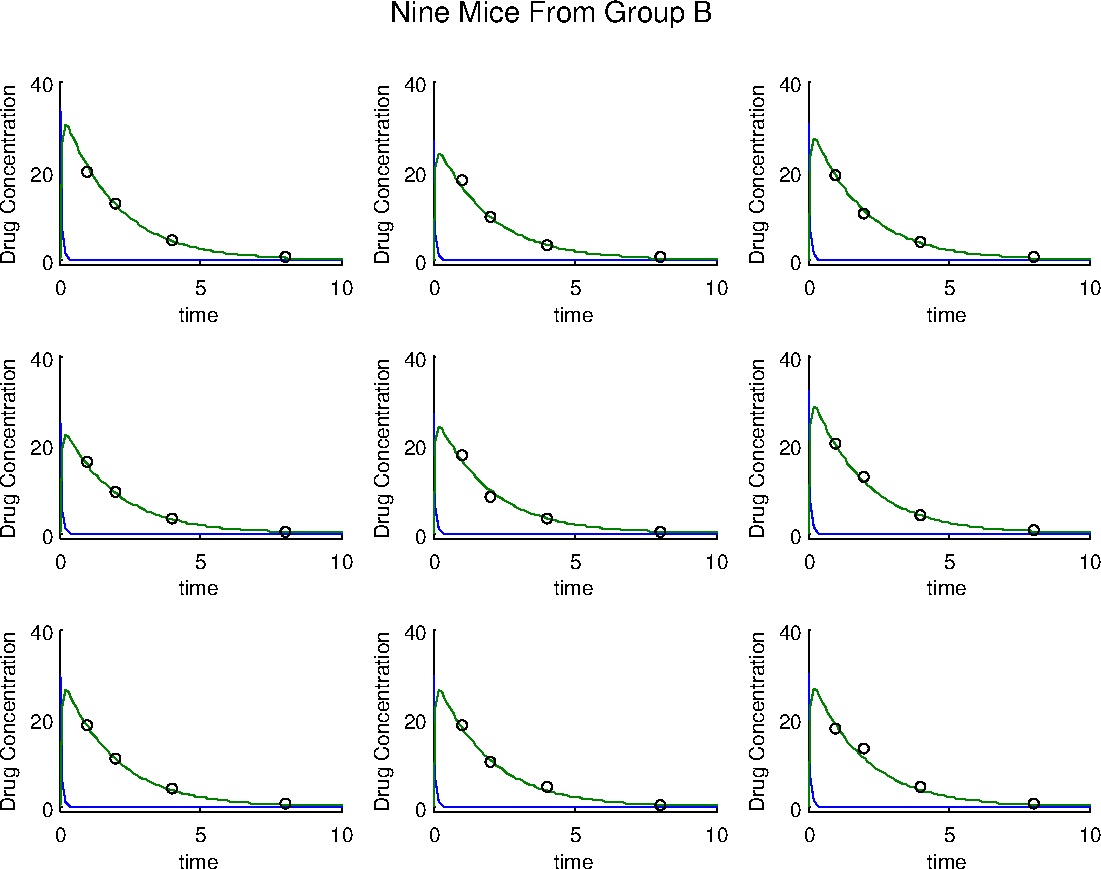
\includegraphics[width=\textwidth]{group_b_plotmatrix.pdf}
\end{frame}
\begin{frame}
  \frametitle{Model Fits}
  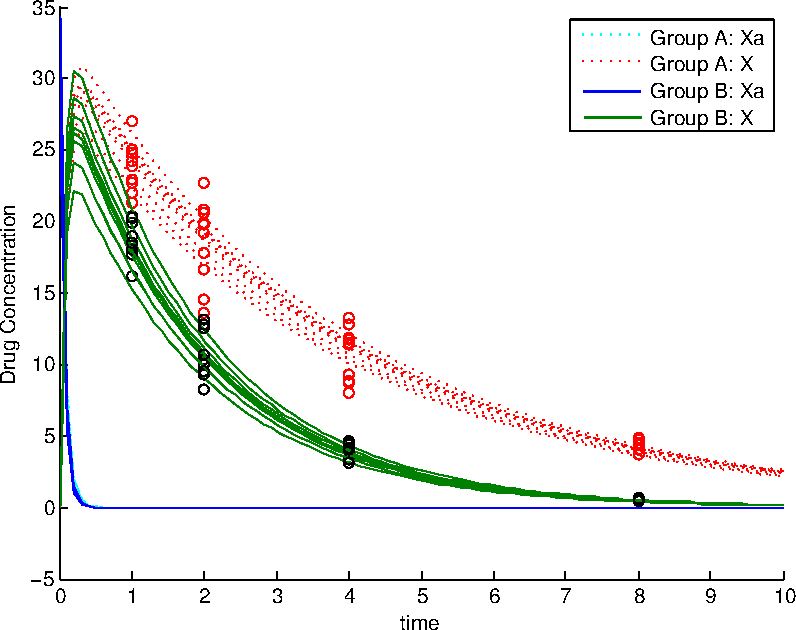
\includegraphics[width=\textwidth]{all_fitted.pdf}
\end{frame}

\begin{frame}[t]
  \frametitle{MCMC Results}
  \begin{columns}
  \column{.55\textwidth}
  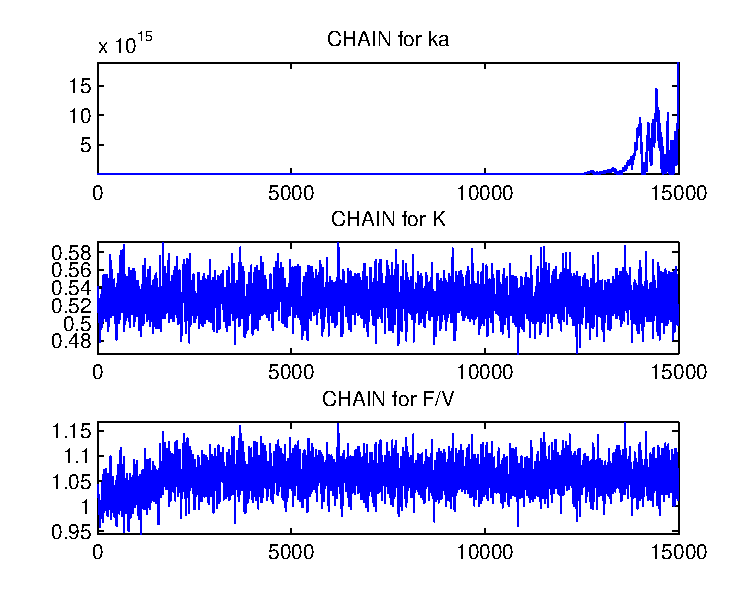
\includegraphics[width=.85\textwidth]{mice_b_chains.pdf} \\
  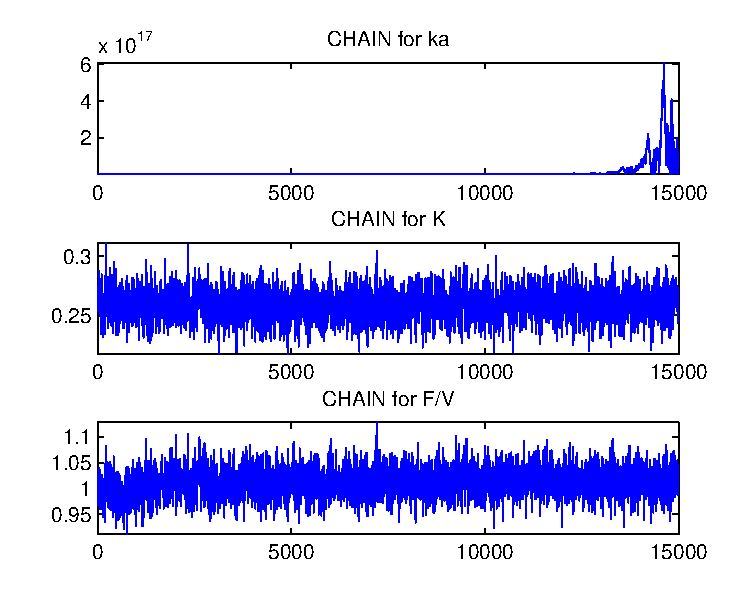
\includegraphics[width=.85\textwidth]{mice_a_chains.pdf}

  \column{.45\textwidth}
  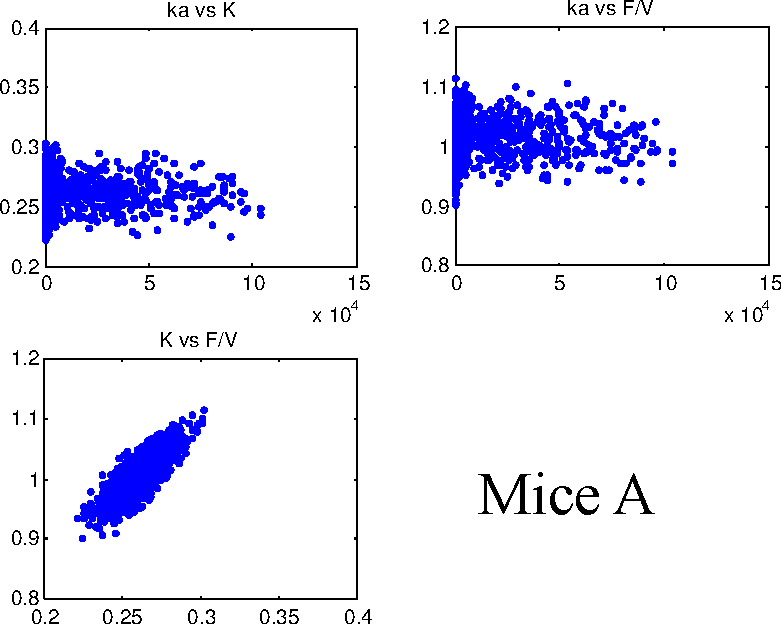
\includegraphics[width=\textwidth]{mice_a_joint_dists.pdf} \\
  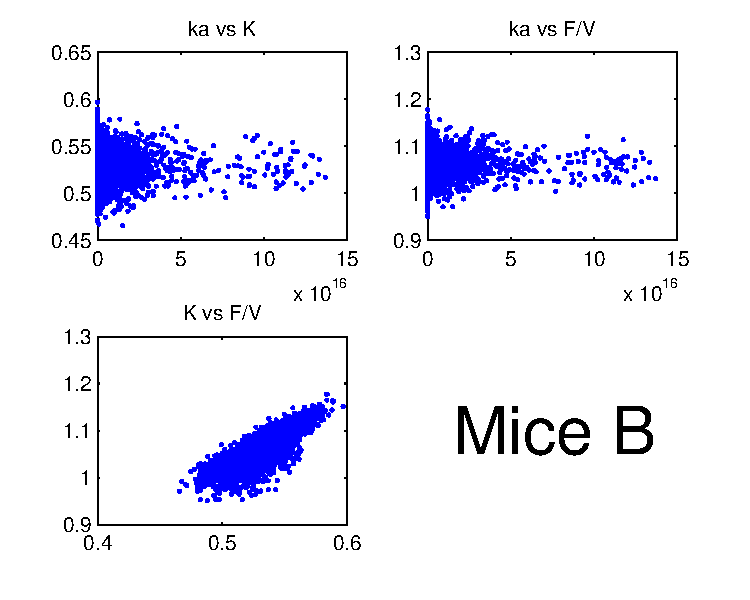
\includegraphics[width=\textwidth]{mice_b_joint_dists.pdf}
  \end{columns}

\end{frame}

%%%%%%%%%%%%%%%%%%%%%%%%%%%%%%%%%%%%%%%%%%%%%%%%%%%%%%%%%%%%%%%%%%%%%%%%%
\section{Conclusion}
\begin{frame}[t]
  \frametitle{Parameter Differences}
  \begin{columns}[T]
  \column{.55\textwidth}
  \includegraphics[width=\textwidth]{drug_abs_diff.pdf} 
  \column{.40\textwidth}
  \vspace{2cm}
  95 \% Confidence Interval:$ [-0.1187,\quad    0.0353]$.
  \end{columns}
  \pause
  Conclusion:  There is insufficient evidence to suggest a difference in the \alert{drug absorption} between the genetically modified and control mice.
  
\end{frame}

\begin{frame}
  \frametitle{Parameter Differences}
  \begin{columns}[T]
  \column{.55\textwidth}
  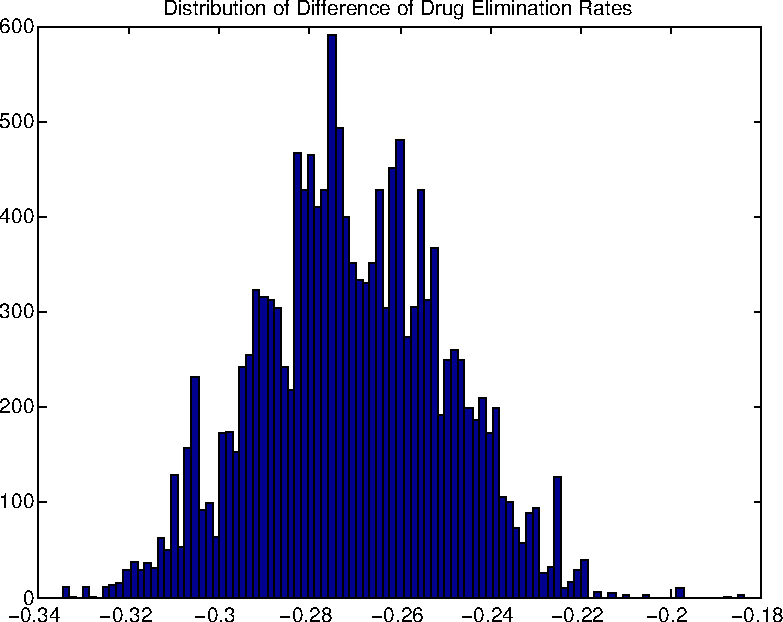
\includegraphics[width=\textwidth]{elim_rate_diff.pdf}
  \column{.45\textwidth}
    \vspace{2cm}
    95 \% Confidence Interval: $[-0.3101,\quad -0.2296]$
  \end{columns}
  \pause
  Conclusion:  There is strong evidence to suggest a difference in the \alert{drug elimination rate} between the genetically modified and control mice.
\end{frame}
%%%%%%%%%%%%%%%%%%%%%%%%%%%%%%%%%%%%%%%%%%%%%%%%%%%%%%%%%%%%%%%%%%%%%%%%%
\end{document}
